% Settings for the default beamer theme
\documentclass[english, aspectratio=169]{beamer}
\usepackage[T1]{fontenc}
\usepackage[utf8]{inputenc}
\usepackage{tabularx}
\usepackage{babel}
\setcounter{secnumdepth}{3}
\setcounter{tocdepth}{3}

\makeatletter

\newcommand\makebeamertitle{\frame{\maketitle}}

% (ERT) argument for the TOC
\AtBeginDocument{%
  \let\origtableofcontents=\tableofcontents
  \def\tableofcontents{\@ifnextchar[{\origtableofcontents}{\gobbletableofcontents}}
  \def\gobbletableofcontents#1{\origtableofcontents}
}

% Theme settings
\usetheme{Frankfurt}
\usecolortheme{default}
\usefonttheme[onlymath]{serif}

% Template settings
\setbeamertemplate{navigation symbols}{}
\setbeamertemplate{blocks}[rounded][shadow=false]
\setbeamertemplate{title page}[default][colsep=-4bp, rounded=true, shadow=false]
\makeatother

\begin{document}

% Title page
\section{Bevezetés}
\title[]{Üzleti Intelligencia}
\subtitle{1. Előadás: Verziókezelés és dokumentálás}
\author[Kuknyó Dániel]{Kuknyó Dániel\\Budapesti Gazdasági Egyetem}
\date{2023/24\\1.félév}
\makebeamertitle

% Table of contents slide
\begin{frame}{Tartalom}
\tableofcontents{}
\end{frame}

\section{Verziókezelés alapfogalmai}

\begin{frame}{Verziókezelés alapjai}
\begin{columns}
\begin{column}{0.5\textwidth}
Miért van szükség verziókezelésre?
\begin{itemize}
	\item A program változásainak követése
	\item A munka biztonságos elmentése
	\item Kollaboráció több fejlesztő között
	\item Programkód párhuzamos szerkesztése
	\item Feladatok szétosztása és követése
\end{itemize}
\end{column}
\begin{column}{0.5\textwidth}
\begin{center}
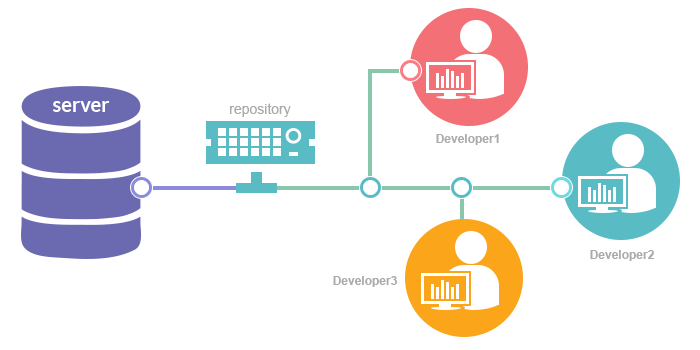
\includegraphics[width=7cm, keepaspectratio]{images/version_control.png}	
\end{center}
\end{column}
\end{columns}
\end{frame}

\begin{frame}{Lokális verziókezelők}
\begin{columns}
\begin{column}{0.5\textwidth}
A legegyszerűbb verziókezelés, ha a fejlessztő kézzel átmásol egy mappába fájlokat. Ezek lehetnek időbélyegzett mappák is, ha okos a fejlesztő. Ez a megoldás nagyon egyszerű, viszont fogékony a hibákra, mert sok a manuális munka. Ezenkívül sok benne a redundáns adat is, mert a nem változtatott adatot is el kell tárolni.  
Ezért hozták létre a lokális verziókezelőket, amik a teljes fájlok helyett csak a változtatásokat tárolták el egy külön erre kifejlesztett adatbázisban. Egy gyakori ilyen szoftver volt az RCS.
\end{column}
\begin{column}{0.5\textwidth}
\begin{center}
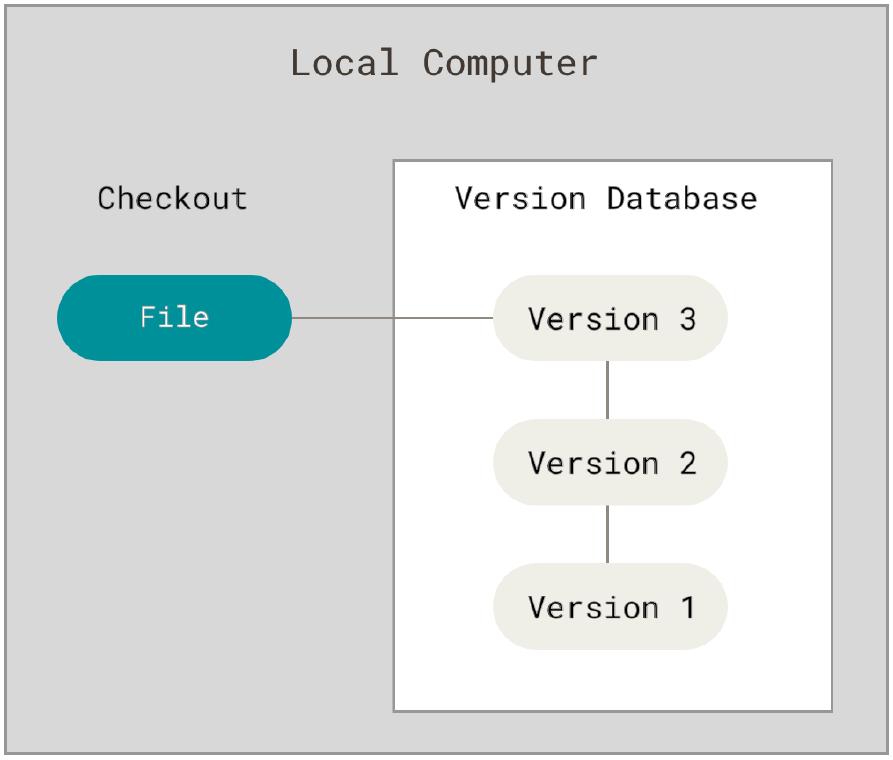
\includegraphics[width=7cm, keepaspectratio]{images/local_vcn.png}
\end{center}
\end{column}
\end{columns}
\end{frame}

\begin{frame}{Centralizált verziókezelők}
\begin{columns}
\begin{column}{0.5\textwidth}
\only<1>{A következő jelentős probléma, amivel az emberek találkoznak, az az, hogy együtt kell működniük fejlesztőkkel más rendszereken. Ennek a problémának a kezelésére Központosított Verziókezelő Rendszerek (CVCS-ek) lettek kifejlesztve. Ezek a rendszerek (például CVS, Subversion és Perforce) egyetlen szerverrel rendelkeznek, amely tartalmazza az összes verziózott fájlt, és számos ügyfél, akik a fájlokat ebből a központi helyről töltik be.}
\only<2>{Előnyei:
\begin{itemize}
	\item Mindenki bizonyos mértékben tudja, hogy a projekt többi résztvevője mit csinál.
    \item Az adminisztrátorok részletes ellenőrzést gyakorolhatnak arról, hogy ki mit tehet meg, és sokkal könnyebb egy CVCS-t adminisztrálni, mint helyi adatbázisokkal foglalkozni minden kliens esetében.
\end{itemize}}
\only<3>{Hátrányai:
\begin{itemize}
	\item Az egyetlen központi szerver hibapontot jelent, ahol akár egy órás leállás is lehetetlenné teszi a közös munkát és verziózási változtatások mentését.
    \item Adatvesztés veszélye, ha a központi adatbázis merevlemeze meghibásodik és nem rendelkezünk megfelelő biztonsági mentésekkel.
\end{itemize}}
\end{column}
\begin{column}{0.5\textwidth}
\begin{center}
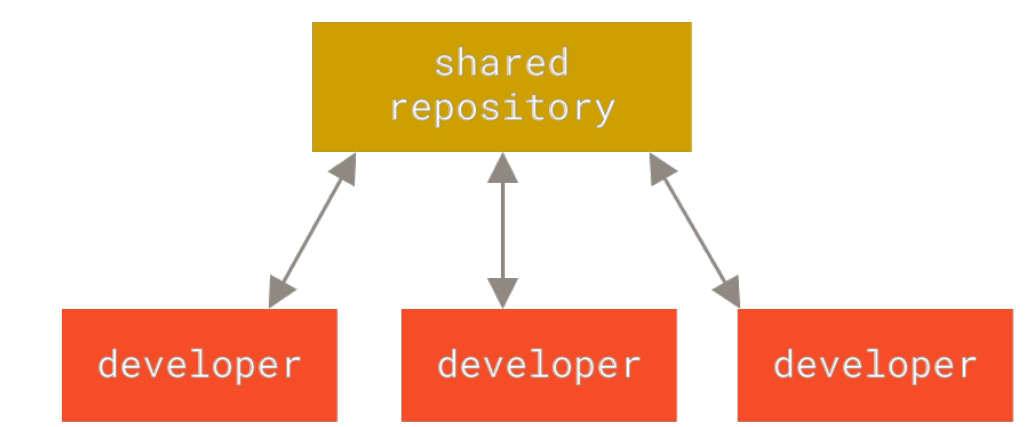
\includegraphics[width=7cm, keepaspectratio]{images/shared_vcn.png}
\end{center}
\end{column}
\end{columns}
\end{frame}

\begin{frame}{Elosztott verziókezelők}
\begin{columns}
\begin{column}{0.5\textwidth}
Ebben a helyzetben lépnek képbe az elosztott verziókezelő rendszerek (DVCS-ek). Egy DVCS-ben a kliensek nem csak a fájlok legfrissebb pillanatképét töltik le, hanem teljes egészében tükrözik a tárhelyet, beleértve annak teljes előzményeit is. Ezért minden klón valójában egy teljes adatbiztonsági másolat.\\
Sok ilyen rendszer nagyon jól kezeli a több távoli tárolóval való együttműködést, így lehetőség van különböző emberekkel egyidejűleg egyazon projekt keretein belül együttműködni.
\end{column}
\begin{column}{0.5\textwidth}
\begin{center}
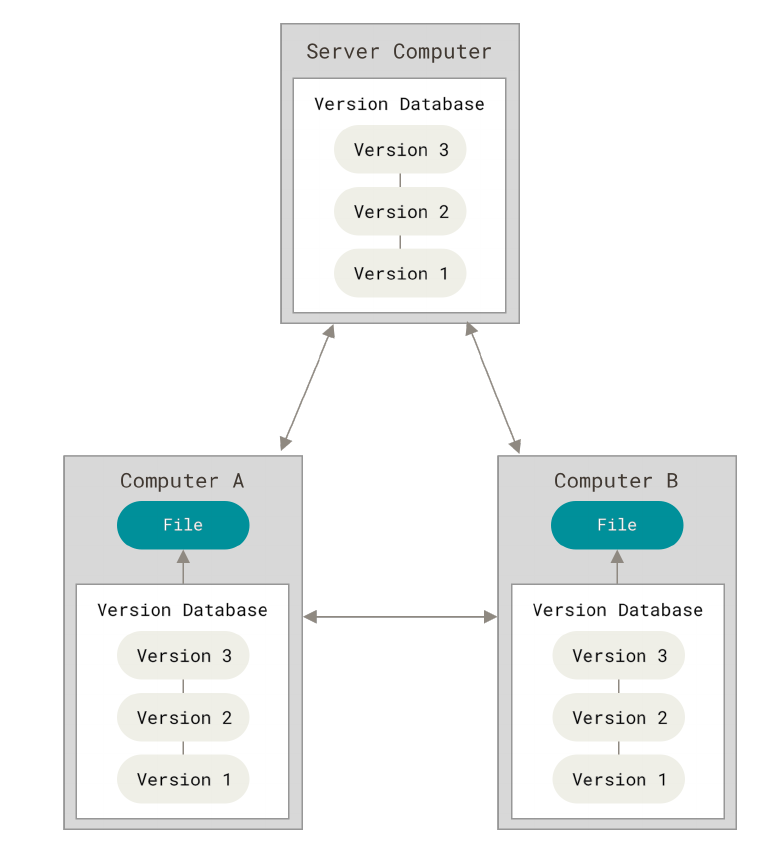
\includegraphics[height=7cm, keepaspectratio]{images/distributed_vcs.png}
\end{center}
\end{column}
\end{columns}
\end{frame}

\section{Git alapok}

\begin{frame}{A Git verziókezelő}
\begin{columns}
\begin{column}{0.5\textwidth}
A Git úgy gondolkodik az adatokról, mint egy fájlrendszer pillanatképei. 
\\Segítségével minden alkalommal, amikor commit történik, (azaz elmentődik a projekt) készít egy képet arról, hogy az összes fájl hogyan néz ki abban a pillanatban, és eltárol egy hivatkozást erre a pillanatfelvételre.\\
A hatékonyság érdekében, ha a fájlok nem változtak, a Git nem tárolja újra a fájlt, csak egy hivatkozást az előző, azonos fájlra, amit már tárolt.
\end{column}
\begin{column}{0.5\textwidth}
\begin{center}
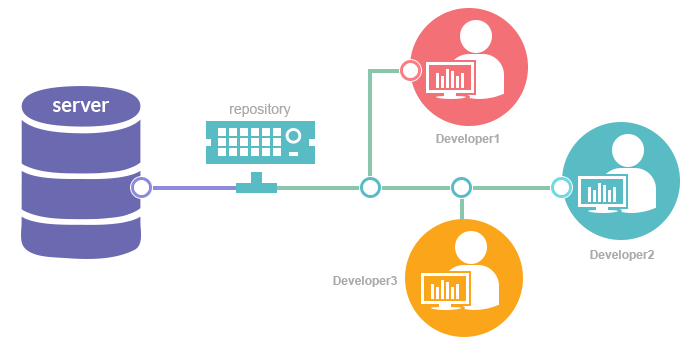
\includegraphics[width=7cm, keepaspectratio]{images/git_1.png}
\end{center}
\end{column}
\end{columns}
\end{frame}

\begin{frame}{A három fájlállapot}
\begin{columns}
\begin{column}{0.5\textwidth}
A Git rendszerében három fő állapota van a fájloknak: módosított (modified), megjelölt (staged) és tárolt (committed):
\begin{itemize}
	\item A módosított azt jelenti, hogy a fájl meg lett változtatva, de még nem lett tárolva, sem tárolásra megjelölve
	\item A megjelölt állapot azt jelenti, hogy a módosított fájl az aktuális verziójában meg lett jelölve, hogy a következő commit pillanatképbe kerüljön
	\item A tárolt azt jelenti, hogy az adat biztonságosan tárolva van a helyi adatbázisban
\end{itemize}
\end{column}
\begin{column}{0.6\textwidth}
\begin{center}
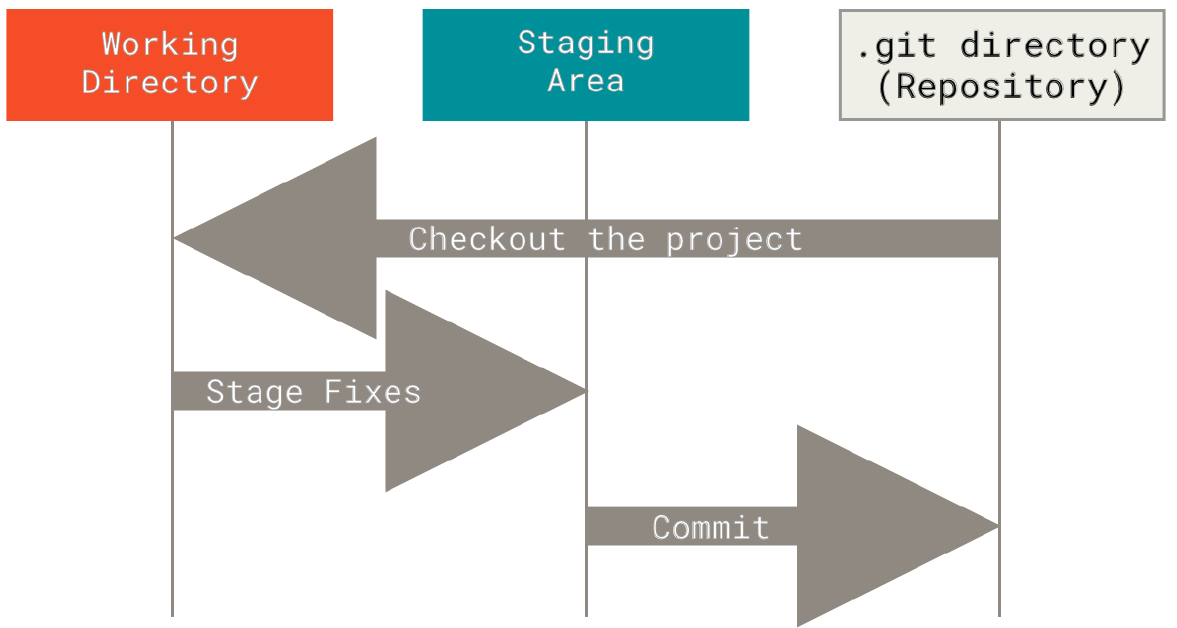
\includegraphics[width=8cm, height=8cm, keepaspectratio]{images/git_2.png}
\end{center}
\end{column}
\end{columns}
\end{frame}

\begin{frame}{Státuszok változása}
\begin{center}
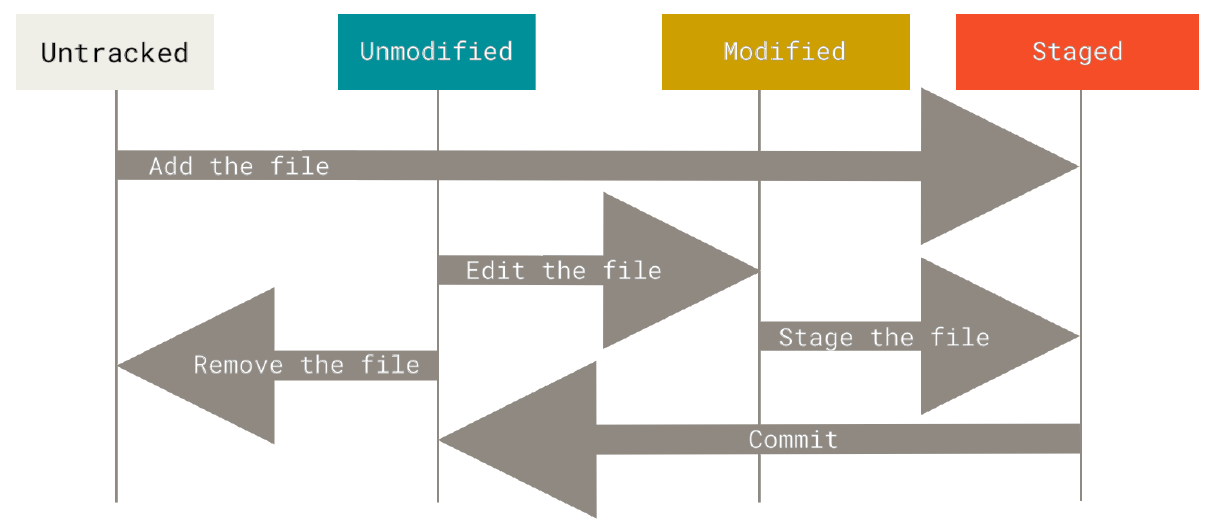
\includegraphics[width=14cm, keepaspectratio]{images/git_3.png}
\end{center}
\end{frame}

\section{Git elágazások}

\begin{frame}{Commitok tárolása}
\begin{columns}
\begin{column}{0.3\textwidth}
\only<1>{Amikor létrehozod a commitot a \textbf{git commit} futtatásával, a Git  faobjektumként tárolja azokat az adattárházban.\\
Ezután a Git létrehoz egy \textbf{commit objektumot}, amely a metaadatokat és egy mutatót tartalmaz a gyökérprojekt fához, így azt újra létre tudja hozni szükség esetén.}
\only<2>{A Git adattárház most öt objektumot tartalmaz: 
\begin{itemize}
	\item Három \textbf{blobot} (amelyek mindegyike egy-egy fájl tartalmát képviseli)
	\item Egy faobjektumot, amely felsorolja a könyvtár tartalmát és megadja, hogy mely fájlnevek tárolódnak mely blobokként
	\item Egy commitot a gyökérfa mutatójával és a metaadatokkal
\end{itemize}}
\end{column}
\begin{column}{0.7\textwidth}
\begin{center}
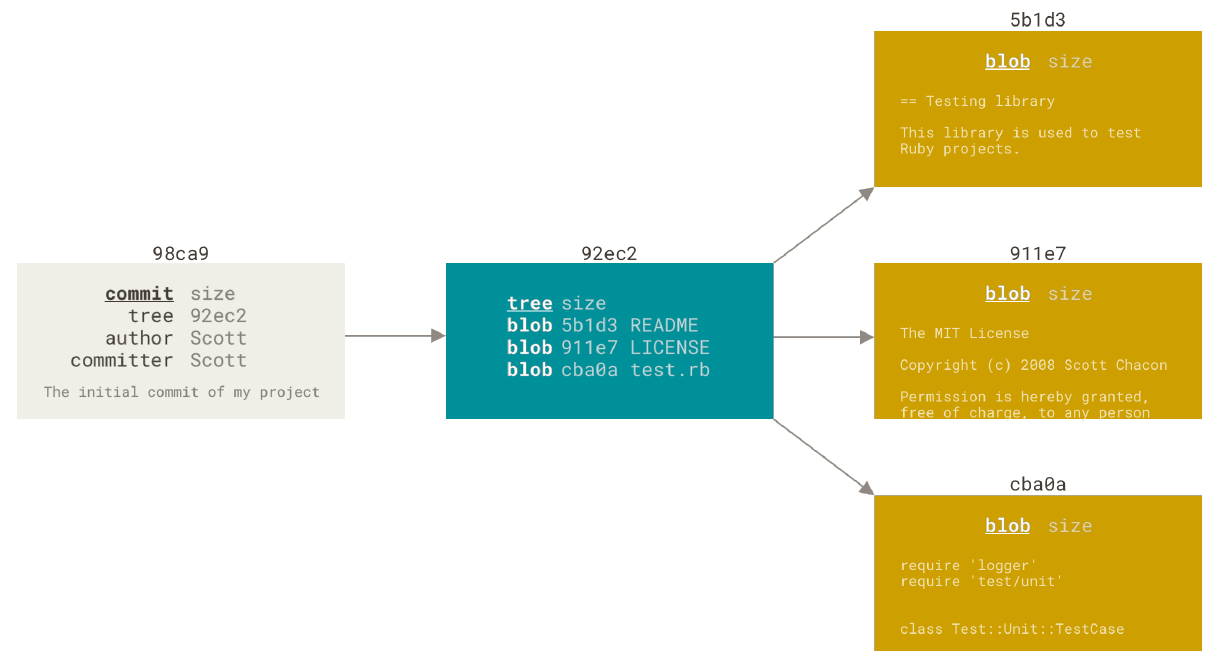
\includegraphics[width=10cm, height=10cm, keepaspectratio]{images/git_4.png}
\end{center}
\end{column}
\end{columns}
\end{frame}

\begin{frame}{Több commit tárolása}
Ha néhány változtatás után ismét egy commit következik, a következő commit egy mutatót tárol arra a commitra, amely közvetlenül megelőzte.\\
\begin{center}
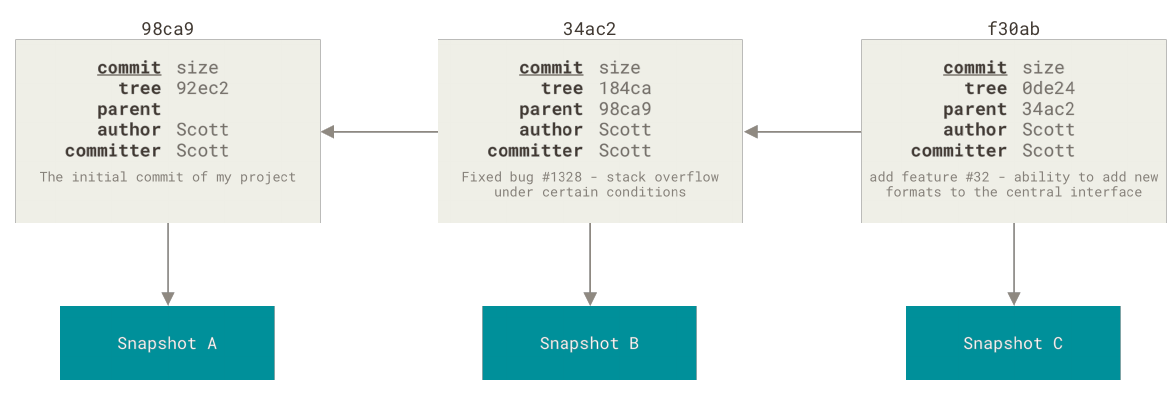
\includegraphics[width=14cm, keepaspectratio]{images/git_5.png}
\end{center}
\end{frame}






\end{document}



















